\documentclass{article}
\usepackage{geometry} % To adjust the margins
\geometry{margin=1in} % Set the margin size
\usepackage{amsmath}
\usepackage{multirow}
\usepackage{multicol}
\usepackage{graphicx} % Required for \resizebox
\usepackage{tikz}
\usepackage{colortbl}
\usepackage{amsmath}

\begin{document}

\vfill % Pushes the content below to the middle of the page

\begin{center}
\Huge \textbf{CSE 210}\\
\vspace{0.5cm}
\LARGE \textbf{Computer Architecture Sessional}\\
\vspace{0.5cm}
\LARGE \textbf{Assignment-1: 4-bit ALU Simulation}
\vspace{2cm}

\LARGE \textbf{Section - C2}\\
\LARGE \textbf{Group - 04}

\vspace{2cm}

\LARGE \textbf{Members of the Group:}

\vspace{0.5cm}

\LARGE
\begin{itemize}
    \item \textbf{2105155} - Md. Siam Ahamed
    \item \textbf{2105158} - Al Shahriar Alif
    \item \textbf{2105160} - Imdadul Hasan Hamim
    \item \textbf{2105172} - Mezba-Us-Salaheen
\end{itemize}
\end{center}

\vfill % Pushes the content above to the middle of the page
\pagebreak


\Large

\section{Introduction}

 ALU, elaborated as Arithmetic and Logic Unit, is quite simply the mathematical brain of a
 computer. It is mainly a combinational digital circuit that performs arithmetic and bitwise
 and logical operations on integer binary numbers. Needless to say, it is a core building block
 of any computing unit, ranging from Central Processing Unit (CPU) to Graphics Processing
 Unit (GPU)s.\\
 
 As the name suggests, an ALU comprises of two main units: Arithmetic Unit and Logic Unit.
 It supports a wide range of operations including arithmetic ones like addition, subtraction,
 increment, decrement, transfer, and logical ones like NOT, OR, XOR, AND etc. The control
 unit routes the source information from registers into ALU inputs. To select a particular
 operation, an ALU has some selection lines or bits. Decoding system allows to support $2^k$
 different operations for k selection lines or bits. In our implemented ALU, there are 3 control
 selection inputs.\\
 
 A parallel adder is the heart of the arithmetic part of the ALU. Multiplexed inputs to the
 IC paves the way to achieve expected results for varieties of arithmetic operations. Besides,
 logical operations can be performed with their respective ICs, and in some efficient designs,
 a particular IC is used to do a different operation other than its intended one.
 There are also 4 status outputs (flags) in our designed ALU. They are denoted by C(Carry
 Flag), Z(Zero Flag), V(Overflow Flag), S(Sign Flag). Their representations carry out the
 following meanings:\\



% Ensuring proper formatting of the descriptions after the colon.
\noindent
\textbf{C}: \hspace*{0.5cm} \parbox[t]{5in}{\textbf{C} is simply the $C_{out}$ of the adder used in the ALU. So, any carry out results in it being 1, otherwise it is set to 0. Logical operations cause it to be 0.}\\[0.5cm]

\noindent
\textbf{Z}: \hspace*{0.5cm} \parbox[t]{5in}{If the last operation of the ALU yielded an output of 0, \textbf{Z} is set, else it is 0.}\\[0.5cm]

\noindent
\textbf{V}: \hspace*{0.5cm} \parbox[t]{5in}{If after any arithmetic operation, two positive numbers result in a negative output, or two negative numbers result in a positive output, that is an overflow and \textbf{V} is set. After any logical operation, it is cleared.}\\

\begin{align}
S_3 &= A_3 \oplus I_3 \oplus C_3 \notag \\
\Rightarrow C_3 &= S_3 \oplus A_3 \oplus I_3 \tag{1} \label{eq-1}\\
V &= C_3 \oplus C_{out} \tag{2}  \label{eq-2}\\
\text{Combining \ref{eq-1} and \ref{eq-2}}  \notag\\
V &= A_3 \oplus I_3 \oplus S_3 \oplus C_{out} \tag{3}
\end{align}


\noindent
 \textbf{S}: It reflects the output MSB.\\



\pagebreak

\Large
\section{Problem Specification with Assigned Instructions}

Design a 4-bit ALU with three selection bits cs0, cs1 and cs2 for performing the following operations:\\

% Adjusting font size and resizing the table
\begin{table}[h!]
\centering
\resizebox{\textwidth}{!}{ % Resize to the text width while maintaining aspect ratio
\begin{tabular}{|c|c|c|l|l|}
\hline
\multicolumn{3}{|c|}{Control Signals} & \multirow{2}{*}{Functions} & \multirow{2}{*}{Boolean Expression} \\ \cline{1-3}
cs2 & cs1 & cs0 &  &  \\ \hline
X   & 0   & 0   & AND              & $A \cap B$             \\ \hline
X   & 0   & 1   & Decrement A       & $A - 1$               \\ \hline
0   & 1   & 0   & Add with Carry    & $A + B + 1$           \\ \hline
0   & 1   & 1   & Subtract          & $A - B$               \\ \hline
1   & 1   & 0   & Complement A      & $A'$                  \\ \hline
1   & 1   & 1   & Transfer A        & $A$                   \\ \hline
\end{tabular}
} % End of resizebox
\label{Table-question}
\caption{ Problem Specification}
\end{table}


\begin{figure}[h!]
\centering
\includegraphics[width=1\textwidth]{4BitALU_blockDiagram.png} % Replace with your image file name
\caption{ 4-bit ALU}
\label{fig-1}
\end{figure}


\pagebreak
\Large

\section{Detailed Design Steps with K-maps}
    \subsection{Design Steps}
        \begin{enumerate}
            \item The arithmetic unit computes four arithmetic operations (Decrement A, Add with Carry, Subtract, and Transfer A) using a 4-bit full adder and a multiplexer.
            \item For the adder, the first input A is fixed, while the second input is either B or \( c \), selected by a multiplexer with the selection bit \( S_1 \). For the Decrement A and Transfer A operations, \( c \) is selected, where \( c = 1111 \) for Decrement A and \( c = 0000 \) for Transfer A. For Add with Carry and Subtract operations, \( B \) and \( B' \) are selected, respectively.
            \item In the arithmetic unit, for the Decrement operation, the adder adds \( A \) with \( c = 1111 \) and \( C_{\text{in}} = 0 \), effectively resulting in \( A - 1 \) in signed representation. For the Transfer operation, \( c = 0000 \) and \( C_{\text{in}} = 0 \), so the adder outputs \( A + 0 = A \). To perform Add with Carry and Subtract operations, the adder adds \( A \) with \( B \) and \( B' \), respectively, with \( C_{\text{in}} \) set to 1 in both cases.
            \item The logical unit performs two logical operations: AND and Complement A. It uses one AND gate and one NOT gate. The output of the logical unit (AND or Complement) is selected by a multiplexer with the selection bit \( S_0 \) (0 for Complement, 1 for AND).
            \item A multiplexer selects the final output of the ALU. When the selection bit \( S_2 = 0 \), the output of the arithmetic unit is selected as the final output, and when \( S_2 = 1 \), the output of the logical unit is selected.
            \item The overflow flag, \( V \), and carry flag, \( C \), are computed from the arithmetic unit. During logical operations, \( C_{\text{in}} = 0 \) and \( c = 0000 \) are selected as the second input to the adder, so there is no chance of overflow or carry, keeping \( V = 0 \) and \( C = 0 \) for logical operations.
            \item The zero flag, \( Z \), is computed by adding the four output bits using three OR gates and then inverting \( O_0 + O_1 + O_2 + O_3 \) with an XOR gate, \( X \oplus 1 = \overline{X} \).
        \end{enumerate}
  \subsection{K-Maps}

To determine the intermediate selection bits $S_0$, $S_1$, and $S_2$, we will use the following K-maps and their corresponding simplified equations:
        

\subsubsection{Solving the K-map for $S_0$:}

The bit $S_0$ serves as the selection input for the multiplexer, which determines the first input to the adder in the arithmetic unit. There are three possible choices for the adder’s first input: $AB$, $A$, or $\overline{A}$. Here’s how each selection works:

$AB$: Selected in case of the AND operation, using both inputs.\\
$A$: Selected for operations like Decrement $A$, Add with Carry, Subtraction, and Transfer.\\
$\overline{A}$: Selected in the Complement $A$ operation.

\begin{center}
    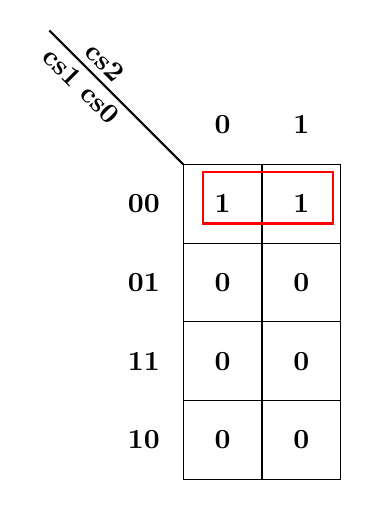
\begin{tikzpicture}
    % Draw the main grid for K-map
    \draw (0,0) grid (2,4);

    % Labels for rows and columns
    \node at (-0.5,3.5) {\textbf{00}};
    \node at (-0.5,2.5) {\textbf{01}};
    \node at (-0.5,1.5) {\textbf{11}};
    \node at (-0.5,0.5) {\textbf{10}};
    \node[rotate=-45] at (-1,5.3) {\textbf{\normalsize cs2}};
    \node[rotate=-45] at (-1.3,5) {\textbf{\normalsize cs1 cs0}};
    \node at (0.5,4.5) {\textbf{0}};
    \node at (1.5,4.5) {\textbf{1}};

    % Values inside the cells
    \node at (0.5,3.5) {\textbf{1}};
    \node at (1.5,3.5) {\textbf{1}};
    \node at (0.5,2.5) {\textbf{0}};
    \node at (1.5,2.5) {\textbf{0}};
    \node at (0.5,1.5) {\textbf{0}};
    \node at (1.5,1.5) {\textbf{0}};
    \node at (0.5,0.5) {\textbf{0}};
    \node at (1.5,0.5) {\textbf{0}};

    % Diagonal line for cs2cs1
    \draw[thick] (-1.7,5.7) -- (0,4);

    % Red rectangle around the first two cells
    \draw[red, thick] (0.25,3.25) rectangle (1.9,3.9);
    \end{tikzpicture}
\end{center}

Based on the K-map, there are two minterms for $S_0$, which we can simplify. Thus, the minimized equation for $S_0$ is:

\begin{center}
    $$
        S_0 = \overline{\text{CS}_1} \, \overline{\text{CS}_0}
    $$
\end{center}
This simplified equation represents the condition under which the multiplexer selects the input for the adder. To clarify how we select among the three options $AB$, $A$, and $\overline{A}$ using a $2 \times 1$ multiplexer:

In this setup, we send the following signals to the two inputs of the multiplexer:

For the first input, we use the expression $A \oplus ({CS}_2 {CS}_1 \overline{{CS}_0})$. This means that when ${CS}_2 = 1$, ${CS}_1 = 1$, and ${CS}_0 = 0$, the expression evaluates to $\overline{A}$; in all other cases, it evaluates to $A$. Thus, we can dynamically select between $A$ and $\overline{A}$ based on the control signals.
For the second input, we simply send $AB$.
With this configuration, the multiplexer can choose between $AB$ and the result of $A \oplus ({CS}_2 {CS}_1 \overline{{CS}_0})$ as the first input to the adder, allowing us to switch between $AB$, $A$, and $\overline{A}$ as needed for the different operations.

\subsubsection{Solving K-map for $S_1$}
The bit $S_1$ serves as the selection input for the multiplexer, which determines the second input to the adder in the arithmetic unit. There are four possible choices for the adder’s second input: $B$,$\overline{B}$,$0$, or $1$ . Here’s how each selection works:

$B$: Selected in case of the  Add with Carry operation.\\
$\overline{B}$: Selected for operations like Subtraction
\\$0$:Selected for And, Complement, and Transfer operation.
\\$1$:Selected for Decrement operation\\
\begin{center}
    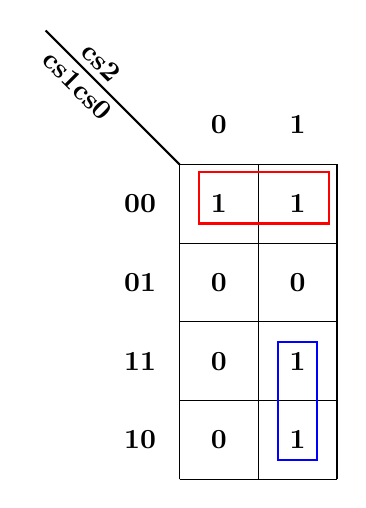
\begin{tikzpicture}
    % Draw the main grid for K-map
    \draw (0,0) grid (2,4);

    % Labels for rows and columns
    \node at (-0.5,3.5) {\textbf{00}};
    \node at (-0.5,2.5) {\textbf{01}};
    \node at (-0.5,1.5) {\textbf{11}};
    \node at (-0.5,0.5) {\textbf{10}};
    \node[rotate=-45] at (-1,5.3) {\textbf{\normalsize cs2}};
    \node[rotate=-45] at (-1.3,5) {\textbf{\normalsize cs1cs0}};
    \node at (0.5,4.5) {\textbf{0}};
    \node at (1.5,4.5) {\textbf{1}};

    % Diagonal label for cs2cs1
    

    % Values inside the cells
    \node at (0.5,3.5) {\textbf{1}};
    \node at (1.5,3.5) {\textbf{1}};
    \node at (0.5,2.5) {\textbf{0}};
    \node at (1.5,2.5) {\textbf{0}};
    \node at (0.5,1.5) {\textbf{0}};
    \node at (1.5,1.5) {\textbf{1}};
    \node at (0.5,0.5) {\textbf{0}};
    \node at (1.5,0.5) {\textbf{1}};
   \draw[thick] (-1.7,5.7) -- (0,4);
   \draw[red, thick] (0.25,3.25) rectangle (1.9,3.9);
    \draw[blue, thick] (1.25,0.25) rectangle (1.75,1.75);
\end{tikzpicture}
\end{center}
Based on the K-map, there are four minterms for $S_1$, which we can simplify. Thus, the minimized equation for $S_1$ is:

\begin{center}
    $$
        S_1 = \overline{\text{CS}_1} \, \overline{\text{CS}_0}+CS_2CS_1
    $$
\end{center}
This simplified equation represents the condition under which the multiplexer selects the input for the adder. To clarify how we select among the four options $B$,$\overline{B}$,$1$ and $0$ using a $2 \times 1$ multiplexer:

In this setup, we send the following signals to the two inputs of the multiplexer:

For the first input, we use the expression  $({CS}_1B \oplus {CS}_0 )$. 
For the second input, we simply send $0$.
With this configuration, the multiplexer can choose between $B$ and the result of $({CS}_1B \oplus {CS}_0 )$ as the second input to the adder, allowing us to switch between $B$,$\overline{B}$, $0$, and $1$ as needed for the different operations.
\subsubsection{Solving K-map for $S_2$}
The selection bit $S_2$ is conventionally used to choose between arithmetic and logical operations. However, in our design, we didn't implement it in this way because switching from arithmetic to logical operations was not necessary due to our design pattern. Our two logical operations, AND and Complement A, are handled directly by manipulating the first input. This approach helped us reduce the number of ICs in our design, making $S_2$ solving a mere formality. Nevertheless, the K-map for $S_2$ is provided here for completeness:
\begin{center}
    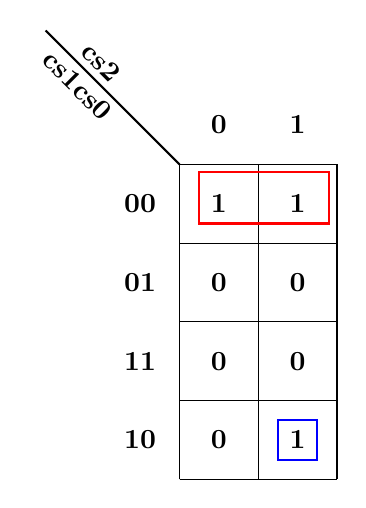
\begin{tikzpicture}
    % Draw the main grid for K-map
    \draw (0,0) grid (2,4);

    % Labels for rows and columns
    \node at (-0.5,3.5) {\textbf{00}};
    \node at (-0.5,2.5) {\textbf{01}};
    \node at (-0.5,1.5) {\textbf{11}};
    \node at (-0.5,0.5) {\textbf{10}};
    \node[rotate=-45] at (-1,5.3) {\textbf{\normalsize cs2}};
    \node[rotate=-45] at (-1.3,5) {\textbf{\normalsize cs1cs0}};
    \node at (0.5,4.5) {\textbf{0}};
    \node at (1.5,4.5) {\textbf{1}};

    % Diagonal label for cs2cs1
    

    % Values inside the cells
    \node at (0.5,3.5) {\textbf{1}};
    \node at (1.5,3.5) {\textbf{1}};
    \node at (0.5,2.5) {\textbf{0}};
    \node at (1.5,2.5) {\textbf{0}};
    \node at (0.5,1.5) {\textbf{0}};
    \node at (1.5,1.5) {\textbf{0}};
    \node at (0.5,0.5) {\textbf{0}};
    \node at (1.5,0.5) {\textbf{1}};
   \draw[thick] (-1.7,5.7) -- (0,4);  
    \draw[red, thick] (0.25,3.25) rectangle (1.9,3.9);
    \draw[blue, thick] (1.25,0.75) rectangle (1.75,0.25);
\end{tikzpicture}

\end{center}
Based on the K-map, we identify three minterms for $S_2$, which we can simplify. The minimized equation for $S_2$ is therefore:
\begin{center}
    $$
        S_2 = \overline{\text{CS}_1} \, \overline{\text{CS}_0}+{{CS}_2}\overline{\text{CS}_0}
    $$
\end{center}

\pagebreak

        
  \section{Truth Table}

For better interpretation of the variables used, refer to Figure 2.

\begin{table}[h!]
    \centering
    \begin{tabular}{|c|c|c|c|c|c|c|c|c|}
        \hline
        \textbf{cs2} & \textbf{cs1} & \textbf{cs0} & \textbf{Function} & \textbf{C\textsubscript{in}} & \textbf{S\textsubscript{0}} & \textbf{S\textsubscript{1}} & \textbf{S\textsubscript{2}} \\
        \hline
        X & 0 & 0 & AND             & 0 & 1 & 1 & 1 \\
        X & 0 & 1 & Decrement A     & 0 & 0 & 0 & 0 \\
        0 & 1 & 0 & Add with carry  & 1 & 0 & 0 & 0 \\
        0 & 1 & 1 & Subtraction     & 1 & 0 & 0 & 0 \\
        1 & 1 & 0 & Compliment A    & 0 & 0 & 1 & 1 \\
        1 & 1 & 1 & Transfer A      & 0 & 0 & 1 & 0 \\
        \hline
    \end{tabular}
    \caption{Truth Table for Intermediate I/O}
\end{table}      
\section{Block Diagram}
\begin{figure}[h!]

\includegraphics[width=1\textwidth]{Blank diagram (1).jpeg} % Replace with your image file name
\caption{ Block Diagram of the circuit}
\label{fig-2}
\end{figure}
\pagebreak
\section{Complete Circuit Diagram}
\begin{figure}[h!]

\includegraphics[width=1\textwidth]{cir.jpg} % Replace with your image file name
\caption{Complete Circuit Diagram}
\label{fig-3}
\end{figure}
\pagebreak
\section{ICs Used with Count as a Chart}
\begin{table}[h!]
\centering
\Large % Change font size here
\begin{tabular}{|l|c|} % Add vertical lines for better clarity
\hline
\textbf{IC} & \textbf{Quantity} \\ 
\hline
IC 7404 & 1 \\ 
IC 7408 & 3 \\ 
IC 7432 & 1 \\ 
IC 7483 & 2 \\ 
IC 7486 & 2 \\ 
IC 74157 & 2 \\ 
\hline
\textbf{Total} & 11 \\ 
\hline
\end{tabular}
\label{Table-IC_count}
\caption{Integrated Circuits Used and Their Counts}
\end{table}

\section{The Simulator Used along with the Version Number}
 Logisim- 2.7.1
\section{Discussion}

 In this assignment, we were tasked to implement a 4-bit ALU which performs 4 arithmetic
 and 2 logical operations.\\
 
 Through rigorous scrutiny, we had to strive hard to obtain the design with the minimum
 number of ICs. In achieving this, we had to make optimizations like performing XOR operation for getting \textbf{V} flag,instead of using a single operation in 7486 IC,we did it in between our extra used adder,7483 IC's extra one port by giving $C_{out}$ in it's A4 pin, 0 in B4 pin and by giving X1,X2,X3 and Y1,Y2,Y3 in previous we got C3.And such,we were able to do $C3 \oplus C_{out} $ and reduce one IC to take place to use. They were results of multiple runs of redoing the
 design.\\

 The hardware implementation also posed challenges like planning the placement of different
 modules. To keep the hardware design clean, we had to connect the wires so that they cross
 as little length as possible between the connections. Extra effort had to be invested to make
 the hardware not just working, but aesthetically pleasing. Power and ground connection
 were done with caution to prevent IC or other components from getting damaged.
 After checking all the boxes, we are hopefully successful in implementing the 4-bit Arithmetic
 and Logic Unit (ALU) with minimum number of ICs.
\section{Contribution of Each Member}

\begin{itemize}
    \item \textbf{Circuit Design:} Imdadul Hasan Hamim (2105160) and Mezba (2105172) led the design and derivation of the circuit, providing the primary framework. Additional support was provided by team members Siam (2105155) and Alif (2105158).
    
    \item \textbf{Circuit Assembly and Arrangement:} Siam (2105155) and Hamim (2105160) handled the input components, while Alif (2105158) and Mezba (2105172) were responsible for the output and flag sections of the circuit.
    
    \item \textbf{Report Writing:} The project report was written by Alif (2105158) and Siam (2105155).
\end{itemize}

\end{document}

